% -*- coding: utf-8 -*-
%%
%%  本模板可以使用以下两种方式编译:
%%     1. PDFLaTeX
%%     2. XeLaTeX [推荐]
%%  注意:
%%    1. 在改变编译方式前应先删除 *.toc 和 *.aux 文件,
%%       因为不同编译方式产生的辅助文件格式可能并不相同。

%\documentclass{cumcmart}
\documentclass[nocover]{cumcmart}%%%切换到无封面的版本,有些区域不允许前面的承诺页用pdf格式,可以用此去掉。



\begin{document}

\xuanti{A}
%\school命令用于在承诺书上显示学校名称。按要求,此处应填写全称
\school{长江大学}
%以下命令分别显示队员及指导教师姓名
\numbers{2017000}%参赛报名号
\authorone{成员一}
\authortwo{成员二}
\authorthree{成员三}
\advisor{数模指导组}

%\theyear{2017}
\theday{20}%填写当月的具体日期

\title{工厂生产最大利润}
\maketitle

% \begin{cnabstract}%此处没有采用sbstract命名,是为了将来如果要加入英文摘要时扩展的方便


% \cnkeywords{差分方程,元胞自动机,交通阻塞模型,数值模拟}
% \end{cnabstract}

% \newpage
%\tableofcontents\newpage%增加目录,要不要都可以。不想要的话,就在本行前加“%”(英文的百分号)


\section{问题重述}

现有三种产品需要经过设备${A_1}$或者${A_2}$的工序${A}$与${B_1}$或者${B_2}$或者${B_3}$的工序${B}$两道工序加工,产品 I 可在 ${A}$,${B}$任何一种规格设备上加工。产品 II 可在任何规格的${A}$设备上加工,但完成${B}$工序时,只能在 ${B_1}$ 设备上加工;产品 III 只能在 ${A_2}$ 与 ${B_2}$设备上加工。已知必要的条件,求使利润最大的最优生产安排。

\section{建模分析}

\subsection{模型假设}
针对该模型,我们提出了如下的合理假设:
\begin{enumerate}
\item 设备在有效台时中不会出现故障;
\item 生产过程连续,即忽略传送产品的时间;
\item 设备生产的产品合格率为${100\%}$;
\item 生产出的产品均以单价售罄。
\end{enumerate}

\subsection{记号说明}
\begin{table}[!htbp]
    \centering
    \begin{tabular}{cl}
    \toprule
    \multicolumn{2}{c}{\large 模型记号说明}\\
    \midrule
    ${c_{ij}}$ &  i产品在j设备上加工的件数 \\
    ${e_{ij}}$ &  i产品在j设备上加工所需要的工时 \\
    ${a_i}$    &  i产品每件获得的利润 \\
    ${b_j}$    &  j设备最大负荷工时 \\
    ${d_j}$    &  j设备满负荷时需要的费用 \\
    \bottomrule
    \end{tabular}
    \caption{模型记号说明}
\end{table}

\subsection{建立模型}
    根据题中所给条件,可以建立线性规划模型 \\
    目标函数
    \[ \max \ Z = \sum_{i=1}^{3}\sum_{j=1}^{5} {\frac{c_{ij}a_{ij}}{2}} - 
    \sum_{i=1}^{3}\sum_{i=1}^{5}{a_{ij}c_{ij}\frac{b_{i}}{d_{i}}} \]
    约束条件
    
    \[ %\begin{equation}
    s.t.
    \left\{  
    \begin{array}{ll}  
    \sum\limits_{i=1}^{2}{c_{ij}} = \sum\limits_{i=3}^{5}{c_{ij}} & j  = 1,2,3  \\ 
     \sum\limits_{i=1}^{3}{c_{ij}e_{ij}} \leqslant b_{i} & i = 1,2 \cdots 5 \\
    \end{array}  
    \right.
    \] %\end{equation} 
    
    即可使用Lingo求解
\subsection{模型求解和分析}
    lingo代码:
    \begin{verbatim}
    model:
    
    SETS:
        number/1..3/:a;
        time/1..5/:b,d;
        link(time,number):c,e;
    ENDSETS
    
    DATA:
        a = 1,1.65,2.3;
        b = 6000,10000,4000,7000,4000;
        d = 300,321,250,783,200;
        e = 5,10,10000,
            7,9,12,
            6,8,10000,
            4,10000,11,
            7,10000,10000;
    ENDDATA
    
    [OBJ] max = @sum(link(i,j):c(i,j)*a(j)/2 - c(i,j)*e(i,j)*d(i)/b(i));
    
    @for(time(i):@sum(number(j):c(i,j)*e(i,j)) <= b(i));
    
    @for(number(j):@sum(time(i)|i#le#2:c(i,j)) =
     @sum(time(i)|i#ge#3:c(i,j)));
    
    @for(link(i,j):@gin(c));
    END
    
    \end{verbatim}
    得到结果:
    
    \begin{figure}
    \centering
    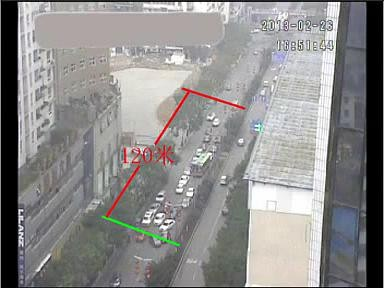
\includegraphics[width=.5\textwidth]{fig1}
    \caption{Lingo求解结果窗口}
    \end{figure}
    
    可以看出最终利润最大为${1146.41}$。
    \begin{figure}
    \centering
    \includegraphics[width=.5\textwidth]{fig3}
    \caption{Lingo求解信息}
    \end{figure}

    \begin{figure}
    \centering
    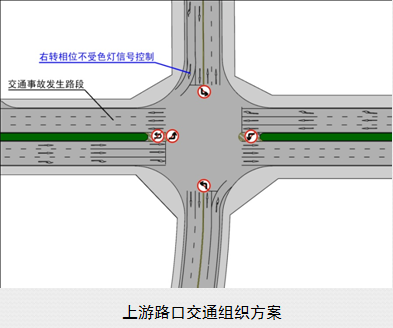
\includegraphics[width=.5\textwidth]{fig2}
    \caption{Lingo所需结果}
    \end{figure}
    可知产品I使用设备${A_1}$加工${1200}$台,设备${A_2}$加工${230}$台,
    设备${B_1}$加工${0}$台,设备${B_2}$加工${859}$台,设备${B_3}$加工${571}$台;
    产品II使用设备${A_1}$加工${0}$台,设备${A_2}$加工${500}$台,
    设备${B_1}$加工${500}$台,不能使用设备${B_2}$、设备${B_3}$加工;
    产品III使用设备设备${A_2}$加工${324}$台,设备${B_2}$加工${324}$台,不能使用设备${A_1}$、设备${B_1}$、设备${B_3}$加工。

\subsection{模型评价}
\subsubsection{模型优点}
1)	

2)	

3)	

\subsubsection{模型缺点}
1)	

2)	


%   \begin{figure}
%   \centering
%   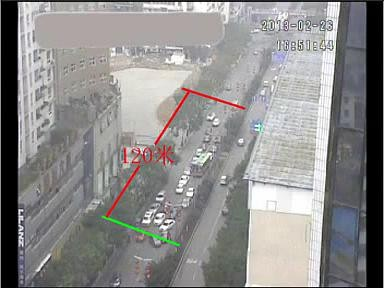
\includegraphics[width=.6\textwidth]{fig1}
%   \caption{发生事故时车流饱和状态图示}
%   \end{figure}

% \begin{thebibliography}{10}
% \bibitem{1} \url{http://bbs.chinatex.org}
% \bibitem{2} \url{http://www.chinatex.org}
% \bibitem{3} Alpha Huang, \textbf{latex-notes-zh-cn}, 2014.
% \bibitem{lf}M.R.C. van Dongen,\textbf{\LaTeX-and-Friends}, 2013.
% \bibitem{figure}Keith Reckdahl,\textbf{Using Import graphics in \LaTeXe}, 1997.
% \bibitem{HM}Addison Wesley,\textbf{Higher Mathematics}, 下载地址如下\\ \url{http://media.cism.it/attachments/ch8.pdf}
% \end{thebibliography}


% \newpage
% \appendix
% \section*{附 \quad 录}


\end{document}
